% Task 7: use bcrypt (black box).
\documentclass[12pt,tikz,border=6pt]{standalone}
% Shared preamble of the task figures of Lecture 7. The colours are the colour roles of the slides
% (main.tex) and of the passwords simulator:
%   Alice sIndigo, Mallory sPink, message / document / password sViolet, salt sAmber,
%   Bob / the server / the notary sTeal, digest sBrown; mechanisms dark; the unknown: orange dashed.
\usepackage{lmodern}
\usepackage[T1]{fontenc}
\renewcommand{\familydefault}{\sfdefault}
\usepackage{amsmath,amssymb}
\usepackage{xcolor}
\usepackage{fontawesome5}
\usetikzlibrary{arrows.meta, calc, positioning, fit, decorations.pathreplacing, backgrounds}

\definecolor{DeepBlue}{HTML}{283593}
\definecolor{AccentOrange}{HTML}{EB5A14}
\definecolor{nInk}{HTML}{37474F}
\definecolor{nLine}{HTML}{90A4AE}
\definecolor{nLight}{HTML}{CFD8DC}
\definecolor{nFill}{HTML}{ECEFF1}
\definecolor{aExec}{HTML}{43A047}
\definecolor{aWrite}{HTML}{E53935}
\definecolor{sIndigo}{HTML}{5C6BC0}
\definecolor{sPink}{HTML}{EC407A}
\definecolor{sViolet}{HTML}{7E57C2}
\definecolor{sAmber}{HTML}{FFB300}
\definecolor{sTeal}{HTML}{26A69A}
\definecolor{sBrown}{HTML}{8D6E63}
\definecolor{sPinkText}{HTML}{C2185B}
\definecolor{sAmberText}{HTML}{A06A00}
\definecolor{sTealText}{HTML}{00796B}

\tikzset{
  hw/.style={draw=nLine, thick, fill=nFill, text=nInk, rounded corners=3pt, align=center, inner sep=4pt},
  mech/.style={draw=nInk, thick, fill=nInk, text=white, rounded corners=3pt, align=center, inner sep=5pt, font=\small\bfseries},
  msgval/.style={draw=sViolet, thick, fill=sViolet!12, text=nInk, rounded corners=3pt, align=center, inner sep=4pt},
  saltval/.style={draw=sAmber, thick, fill=sAmber!25, text=nInk, rounded corners=3pt, align=center, inner sep=4pt},
  digval/.style={draw=sBrown, thick, fill=sBrown!15, text=nInk, rounded corners=3pt, align=center, inner sep=4pt},
  srvval/.style={draw=sTeal, thick, fill=sTeal!15, text=nInk, rounded corners=3pt, align=center, inner sep=4pt},
  unk/.style={draw=AccentOrange, thick, dashed, fill=white, text=AccentOrange, rounded corners=3pt, align=center,
    inner sep=4pt, font=\bfseries},
  data/.style={-{Stealth}, very thick, nInk},
  person/.style={circle, fill=#1, draw=#1, text=white, minimum size=1.1cm, font=\Large, inner sep=0pt},
}
\newcommand{\personnode}[4]{%
  \node[person=#3] (#1) at (#2) {\faUser};
  \node[font=\small\bfseries, text=#3, below=0.06cm of #1] (#1lbl) {#4};}
\newcommand{\mallorynode}[2]{%
  \node[person=sPink] (#1) at (#2) {\faUserSecret};
  \node[font=\small\bfseries, text=sPinkText, below=0.06cm of #1] (#1lbl) {Mallory};}
\newcommand{\hashbox}[4]{\node[mech, minimum width=#4] (#1) at (#2) {\faCogs\ #3};}

\begin{document}
\pagecolor{white}
\begin{tikzpicture}[>=Stealth]
  \personnode{al}{-1.6,0}{sIndigo}{Alice}
  \node[msgval, font=\small\ttfamily] (p) at (1.4,0.8) {blue tulip 42};
  \node[saltval, font=\small] (s) at (1.4,0) {new random salt};
  \node[hw, font=\small] (c) at (1.4,-0.8) {cost = 4};
  \node[mech, minimum width=2.2cm, minimum height=2.2cm, font=\large\bfseries] (b) at (4.8,0) {\faCogs\\ bcrypt};
  \draw[data] (al) -- (p.west);
  \draw[data] (p) -- (b.west |- p);
  \draw[data] (s) -- (b);
  \draw[data] (c) -- (b.west |- c);
  \node[font=\small\ttfamily, anchor=west, align=left] (o1) at (6.4,0.5) {first:\ \ \$2b\$04\$\textcolor{sAmberText}{\textbf{?????}}\textcolor{sBrown}{\textbf{?????}}};
  \node[font=\small\ttfamily, anchor=west, align=left] (o2) at (6.4,-0.5) {second: \$2b\$04\$\textcolor{sAmberText}{\textbf{?????}}\textcolor{sBrown}{\textbf{?????}}};
  \draw[data] (b) -- (6.3,0);
  \node[unk, font=\small] at (10.6,-1.3) {the same text twice?};
  \node[srvval, font=\small, text width=9.0cm, align=left] at (3.4,-2.4) {\faServer\ Bob's server at login:\\ check\_password("blue tulip 42", first) = ?\\ check\_password("blue tulip 43", first) = ?};
\end{tikzpicture}
\end{document}
